\chapter{Methodology}\label{ch:method}

This chapter describes the data, how it was cleaned and joined, the reference that alerts are scored against, the forecast benchmark, the three alert rules, and how every setting was chosen and then scored. The whole pipeline is shown in Figure~\ref{fig:workflow}. Each step is one Jupyter notebook; the code is in a public GitHub repository and the data, which contains TCB prices, stays in a private Google Drive folder.

\begin{figure}[H]
\centering
\begin{tikzpicture}[
  box/.style={draw, rounded corners=2pt, align=center, font=\footnotesize, minimum height=1.0cm, text width=2.5cm},
  key/.style={box, very thick},
  gate/.style={draw, dashed, font=\scriptsize, align=center, inner sep=2pt},
  arr/.style={-{Stealth[length=2mm]}, thick},
  lab/.style={font=\scriptsize, align=center}]
\node[box] (raw) {4 raw files\\TCB prices, Ramadan/Eid,\\exchange rate, weather};
\node[box, right=0.6cm of raw] (n02) {01 intake\\02 processing\\clean, join, check};
\node[key, right=0.6cm of n02] (data) {\texttt{data\_8.csv}\\8 items $\times$ 1,412\\report days};
\node[box, above=0.7cm of data] (n03) {03 price behaviour\\sustained rises};
\node[box, right=0.6cm of data] (n04a) {04a choose forecast\\on 2024};
\node[box, below=0.9cm of n04a] (n04b) {04b score forecasts\\2025-26 \retro};
\node[box, left=0.6cm of n04b] (n05a) {05a choose alert\\settings on 2024};
\node[box, left=0.6cm of n05a] (n05b) {05b score the\\three alert rules};
\node[box, below=0.9cm of n05b] (n06) {06 report tables\\and register};
\node[key, right=0.6cm of n06] (n07) {07 monitor app\\(Gradio)};
\draw[arr] (raw) -- (n02);
\draw[arr] (n02) -- (data);
\draw[arr] (data) -- (n03);
\draw[arr] (data) -- (n04a);
\draw[arr] (n04a) -- node[gate, right] {commit\\8d7c145} (n04b);
\draw[arr] (n04b) -- node[lab, above] {7-day\\forecasts} (n05a);
\draw[arr] (n05a) -- node[gate, above=2pt] {commit\\e0cfa06} (n05b);
\coordinate (L) at ($(raw.west)+(-0.35,0)$);
\draw[arr] (n03.west) -- node[lab, above] {rise episodes (reference)} (n03.west -| L) |- (n05b.west);
\draw[arr] (n05b) -- (n06);
\draw[arr] (n05b) -- node[lab, right] {alerts} (n07);
\end{tikzpicture}
\caption[Workflow of Food Price Watch]{Workflow of Food Price Watch. Each box is one notebook. The dashed labels are commits: a setting chosen on 2024 was written into the settings file and pushed before the notebook that scores 2025-26 was run.}
\label{fig:workflow}
\end{figure}

\section{Data}\label{sec:data}

\subsection{Sources}
The prices come from the daily retail price reports of the Trading Corporation of Bangladesh (TCB) for Dhaka \cite{tcb}. On most working days TCB publishes a sheet that gives, for each item, the lowest and highest retail price seen in Dhaka markets that day, in taka. The sheets from 17 May 2021 to 24 October 2026 had been converted into one long table during an earlier phase of this work and checked against the original files: a machine re-read of 1,530 sampled rows on 28 report days compared 3,060 price cells and found no mismatch. The audit checks the copying only; it cannot show that TCB itself recorded a value correctly.

Three other files are used: Ramadan and Eid dates; the taka per US dollar exchange rate (daily market quotes); and daily weather at 13 locations in Bangladesh from Open-Meteo \cite{openmeteo}. The four raw files are copied once into a \texttt{raw/} folder, never edited, and listed with their sha256 hashes in a manifest.

\subsection{The eight items}
The study covers eight everyday items (Table~\ref{tab:items}). They were chosen because they are common household purchases and because their prices move often enough to study. They were chosen after the results of an earlier, wider run of this project (54 items) had been seen; this is a limitation and is discussed in Section~\ref{sec:threats}. Each item is a product together with its unit, for example eggs per hali (four eggs). The group names come from the earlier run and are used only to describe the items.

\begin{table}[H]\centering\small
\caption[The eight items]{The eight items, their units, groups, the cost drivers used for each, and the share of report days on which the price is missing.}\label{tab:items}
\begin{tabular}{llllr}
\toprule
\textbf{Item} & \textbf{Unit} & \textbf{Group} & \textbf{Drivers used} & \textbf{Not reported (\%)} \\
\midrule
Chicken - Broiler & per kg & volatile perishable & none & 0.00 \\
Egg - Farm & per hali (4 pcs) & volatile perishable & none & 0.07 \\
Onion - Local & per kg & volatile perishable & weather & 0.07 \\
Potato & per kg & domestic staple & weather & 0.07 \\
Garlic - Imported & per kg & imported staple & exchange rate & 0.07 \\
Palm Oil - Loose & per litre & administered & exchange rate & 0.00 \\
Soybean Oil - Loose & per litre & administered & exchange rate & 0.28 \\
Sugar & per kg & administered & exchange rate & 0.00 \\
\bottomrule
\end{tabular}

\source{\path{reports/tables/report/R1_data.csv} (notebook 02).}
\end{table}

\subsection{Data format and shape}
Everything is joined into one table, \texttt{data\_8.csv}, in long format: one row per item and report day. With 8 items and 1,412 report days it has 11,296 rows and 20 columns and no duplicate keys (Table~\ref{tab:columns}). Lags, rolling means and forecast targets depend on the forecast horizon, so they are built from the price inside the forecasting notebooks instead of being stored.

\begin{table}[H]\centering\small
\caption[Columns of the data table]{Columns of \texttt{data\_8.csv}.}\label{tab:columns}
\begin{tabularx}{\linewidth}{>{\raggedright\arraybackslash}p{5.2cm}X}
\toprule
\textbf{Column(s)} & \textbf{Meaning} \\
\midrule
\texttt{Date}, \texttt{item\_id} & report day; item as ``product $|$ unit'' (the key) \\
\texttt{Price\_Min}, \texttt{Price\_Max}, \texttt{Price\_Avg} & lowest and highest Dhaka retail price in the TCB sheet and their midpoint (Tk); blank = not reported \\
\texttt{report\_idx} & report-day number, 0 = 17 May 2021; the time axis for lags and horizons \\
\texttt{gap\_2022} & the day lies in the sparse 2022 period \\
\texttt{days\_since\_prev\_report} & calendar days since the previous TCB sheet \\
\texttt{reports\_since\_change} & report days the price has stayed the same \\
\texttt{month}, \texttt{dow}, \texttt{days\_to\_ramadan}, \texttt{days\_to\_eid\_fitr}, \texttt{days\_to\_eid\_adha}, \texttt{in\_ramadan} & calendar, known in advance \\
\texttt{wx\_tmax\_7d}, \texttt{wx\_tmean\_30d}, \texttt{wx\_rain\_7d} & 7-day maximum temperature, 30-day mean temperature, 7-day rainfall (Bangladesh mean); onion and potato only \\
\texttt{fx\_lvl}, \texttt{fx\_ch30} & log taka per US dollar and its 30-day change; garlic, both oils and sugar only \\
\bottomrule
\end{tabularx}

\end{table}

\subsection{Cleaning rules}
The cleaning follows a small set of fixed rules. None of them invents a price, removes a real one, or uses a value before it was known.
\begin{enumerate}[leftmargin=*,itemsep=2pt]
\item \textbf{Price.} The price of an item on a day is the midpoint $P = (P_{\min} + P_{\max})/2$. TCB reports whole taka, so the midpoint moves in steps of Tk 0.5; every observed change is a multiple of 0.5.
\item \textbf{Missing prices.} A blank or zero price means ``not reported''. This affects 8 of the 11,296 cells. A missing price is never filled in a forecast target and never counted as a zero change. Model inputs may carry the last reported price forward.
\item \textbf{The 2022 gap.} From 12 March to 31 December 2022 TCB published only 24 sheets. These rows are kept and flagged. No price change, rise window, forecast target or model fit spans the gap, and ETS is fitted on data after the gap only.
\item \textbf{Real jumps stay.} There is no outlier removal: a jump in a TCB sheet is exactly what the alerts are meant to see.
\item \textbf{Checks.} Notebook 02 stops if any of these fails: duplicate keys; a midpoint that is not the average of minimum and maximum; minimum above maximum; a zero, negative or infinite price; a driver used before it was available; a driver attached to an item that does not use it.
\end{enumerate}

\subsection{Cost drivers and availability dates}\label{sec:avail}
Two clocks are used. Horizons and lags count \emph{report days}, because TCB does not publish every calendar day: ``seven days ahead'' means seven TCB sheets ahead. Drivers are joined by the \emph{calendar date on which they became known}:
\begin{itemize}[leftmargin=*,itemsep=2pt]
\item Weather of day $d$ is treated as usable from day $d+5$.
\item The exchange rate on a report day is the last quote on or before that day. Its 30-day change uses the last quote on or before the day 30 days earlier. A quote older than 7 days is left empty, never set to zero.
\item Calendar columns (month, weekday, days to Ramadan and the two Eids) are known in advance and may be used at any time.
\end{itemize}
Weather is used only for onion and potato, and the exchange rate only for imported garlic, the two oils and sugar (Table~\ref{tab:items}).

\section{Price behaviour and sustained rises}\label{sec:method-behaviour}

\subsection{Price-change measures}
For each item, notebook 03 measures how often the price changes from one report day to the next, the size of the changes when they happen, how long the price stays unchanged, the smallest price step, and whether prices behave differently in the 30 days before Ramadan. These measures are descriptive. They explain why forecasting these prices is hard, and they say nothing about why prices move.

\subsection{Sustained rise: the reference for scoring alerts}\label{sec:rise}
An alert has to be scored against something that does not depend on any model. The reference is a \emph{sustained rise}, defined from TCB prices alone:
\begin{enumerate}[leftmargin=*,itemsep=2pt]
\item On each report day $t$ the rise ratio is $R_t = P_t / P_{t-14} - 1$, where $t-14$ is 14 report days earlier. Windows that touch the 2022 gap are skipped.
\item Day $t$ is a \emph{rise day} if $R_t \geq 10\,\%$.
\item A \emph{sustained rise episode} is a run of at least 5 consecutive rise days. Episodes of the same item fewer than 14 report days apart are merged. The first rise day is the \emph{onset}.
\end{enumerate}
This rule was fixed in the earlier run before this study started and was not re-chosen. The same counts with 7\,\% and 15\,\% thresholds are reported as a sensitivity check and are never used to choose anything.

\section{Forecast benchmark}\label{sec:method-forecast}
The forecasts are a benchmark: they test whether a model can say something about the next days that \naive{} cannot. Every model forecasts the change in the logarithm of the price over $h$ report days, $y_{t,h} = \log P_{t+h} - \log P_t$, for $h \in \{1, 7, 14, 30\}$. Working in log changes puts an item that costs Tk 20 and one that costs Tk 200 on the same scale.

\subsection{Models}
\begin{itemize}[leftmargin=*,itemsep=2pt]
\item \textbf{Naive (\naive).} The forecast change is zero: the last reported price.
\item \textbf{ETS.} Automatic exponential smoothing \cite{hyndman2002}, fitted to each item's log price after the 2022 gap with the AutoETS function of statsforecast \cite{statsforecast}.
\item \textbf{LightGBM.} One gradient-boosted tree model \cite{lightgbm} for all items and all four horizons, with the horizon as an input. The price-history inputs are the log changes over the last 1, 7, 14 and 30 report days, the deviation of the price from its 30-report mean, the 30-report volatility of daily changes, the number of report days since the price last changed, and the item. The ``price plus drivers'' feature set adds the calendar, weather and exchange-rate columns.
\end{itemize}

\subsection{Training, validation and test}\label{sec:splits}
The data is never shuffled. A forecast is made at a \emph{forecast origin}, and a model fitted for that origin sees only rows whose target lies on or before the origin. The training window expands as time moves on (Figure~\ref{fig:splits}).
\begin{itemize}[leftmargin=*,itemsep=2pt]
\item \textbf{Training:} all history before each origin.
\item \textbf{Validation:} the year 2024, 43 weekly origins. Every choice of model setting, alert level and threshold is made here.
\item \textbf{Test:} 1 January 2025 to 24 October 2026, 82 weekly origins whose 30-day targets all fall on or before the last report day. This period had already been looked at in the earlier run of the project, so its results are called \emph{retrospective} throughout.
\end{itemize}
Origins are 7 report days apart. LightGBM is refitted every 8 origins and reused in between; ETS is refitted at every origin.

\begin{figure}[H]
\centering
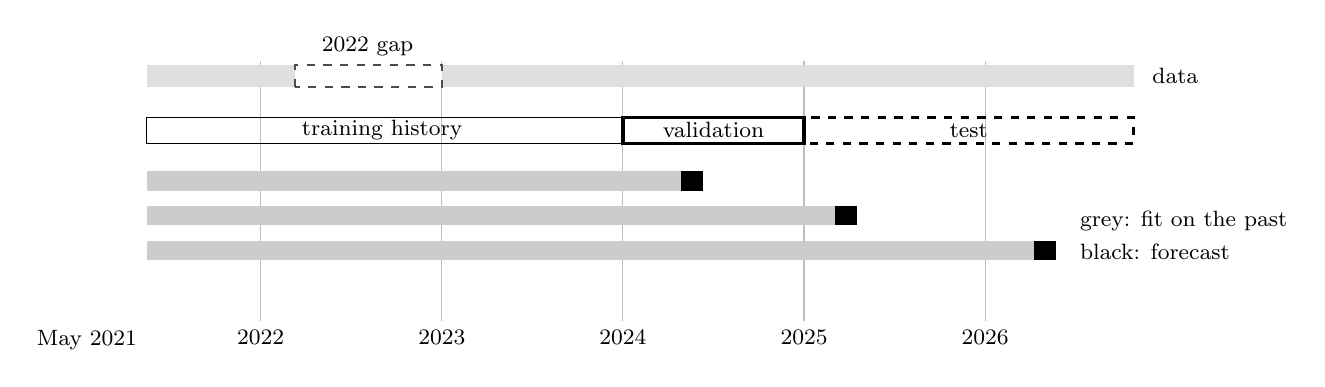
\begin{tikzpicture}[x=2.3cm, y=0.55cm, font=\footnotesize]
\foreach \yr/\x in {2022/0.63, 2023/1.63, 2024/2.63, 2025/3.63, 2026/4.63}{
  \draw[gray!50] (\x,-0.4) -- (\x,5.6); \node[below] at (\x,-0.4) {\yr};}
\node[below left] at (0,-0.4) {May 2021};
\fill[gray!25] (0,5) rectangle (5.45,5.5);
\fill[white] (0.82,5) rectangle (1.63,5.5);
\draw[thick, black!70, dashed] (0.82,5) rectangle (1.63,5.5);
\node[right] at (5.5,5.25) {data};
\node[above] at (1.22,5.5) {2022 gap};
\draw (0,3.7) rectangle (2.63,4.3); \node at (1.3,4) {training history};
\draw[very thick] (2.63,3.7) rectangle (3.63,4.3); \node at (3.13,4) {validation};
\draw[very thick, dashed] (3.63,3.7) rectangle (5.45,4.3); \node at (4.54,4) {test \retro};
\foreach \e/\yy in {2.95/2.6, 3.8/1.8, 4.9/1.0}{
  \fill[gray!40] (0,\yy) rectangle (\e,\yy+0.45);
  \fill[black] (\e,\yy) rectangle (\e+0.12,\yy+0.45);}
\node[right] at (5.1,1.9) {grey: fit on the past};
\node[right] at (5.1,1.2) {black: forecast};
\end{tikzpicture}
\caption[Training, validation and test periods]{Training, validation and test periods. The grey bars show three example forecast origins: the model is fitted on everything before the origin and forecasts the next 1 to 30 report days. The 2022 gap is never crossed.}
\label{fig:splits}
\end{figure}

\subsection{Choosing the LightGBM setting}
Sixteen configurations were compared on 2024: feature set (price only; price plus drivers) $\times$ number of leaves (7; 31) $\times$ learning rate (0.03; 0.05) $\times$ loss (absolute error; Huber), with 300 boosting rounds. The score is the geometric mean, over items and horizons, of the model's MAE divided by the MAE of \naive{}. Configurations were ordered from simplest to most complex, and a simpler one within 1\,\% of the best was preferred. The chosen setting was written into the settings file and committed (commit \texttt{8d7c145}) before the test notebook was written.

\section{The alert system}\label{sec:method-alerts}
The monitor compares each day's price with an \emph{expected range} drawn 7 report days earlier and raises an alert when the price stays above that range. It is abnormal-rise detection: it says that a rise is unusual for that item, not that a rise is coming.

\subsection{The expected range}
Every report day since June 2023 has a 7-report-ahead forecast. For target day $t$, the forecast was made at origin $t-7$. The upper bound adds to that forecast the $q$-quantile of the item's last 120 forecast errors whose targets lay on or before the origin $t-7$. Only errors that were already known at the origin are used, so the range never looks ahead. At least 30 known errors are needed before a range is drawn. This way of building a range from past out-of-sample errors follows Lee and Scholtes \cite{lee2014}.

\subsection{Three rules}
The three rules differ only in how the upper bound is drawn (Table~\ref{tab:rules}). Rule A uses the LightGBM forecast and its errors. Rule B uses \naive{}, so its errors are simply the item's past 7-report price changes. Rule C uses no model at all: it is a fixed percentage rise over 7 report days, the same for every item.

\begin{table}[H]\centering\small
\caption[The three alert rules]{The three alert rules and their candidate settings.}\label{tab:rules}
\begin{tabularx}{\linewidth}{lXl}
\toprule
\textbf{Rule} & \textbf{Upper bound on report day $t$} & \textbf{Candidates} \\
\midrule
A. ML range & LightGBM forecast of the 7-report change made at $t-7$, plus the $q$-quantile of the item's last 120 known LightGBM errors & $q \in \{0.90, 0.95, 0.975, 0.99\}$ \\
B. Simple range & ``no change'' made at $t-7$, plus the $q$-quantile of the item's last 120 known 7-report changes & $q \in \{0.90, 0.95, 0.975, 0.99\}$ \\
C. Fixed rise & price at $t-7$ times $(1+c)$, the same $c$ for every item & $c \in \{3, 5, 7, 10\}\,\%$ \\
\bottomrule
\end{tabularx}

\end{table}

\subsection{From exceedance to alert}
A day is an \emph{exceedance} when the price is above the upper bound. A single exceedance is not an alert: one-day jumps are common and often reverse. An item is in \emph{alert} on day $t$ when it exceeded the bound on at least 3 of its last 5 report days. Consecutive alert days form one \emph{alert run}, and the first day of the run is the day the monitor would report.

\subsection{Choosing the settings on 2024}
For each rule, the candidate settings were scored on 2024. The chosen setting is the most sensitive one whose alert runs that match no sustained rise stay at or below 2 per item-year, where an item-year is 250 report days. The three settings were committed (commit \texttt{e0cfa06}) before the scoring notebook was written.

\section{Evaluation}\label{sec:eval}

\subsection{Forecast accuracy}
\begin{itemize}[leftmargin=*,itemsep=2pt]
\item \textbf{MAE} of the log change, and the MAE of \naive{} on the same targets.
\item \textbf{Relative MAE} = model MAE / \naive{} MAE, combined over items with a geometric mean \cite{hk2006}. Below 1 is better than \naive{}.
\item \textbf{Accuracy} = $1 - $ MAPE. It is shown only next to the accuracy of \naive{}: on prices that rarely move, a high accuracy costs nothing.
\item \textbf{Diebold--Mariano test} \cite{dm1995} with the small-sample correction of Harvey, Leybourne and Newbold \cite{hln1997}, on the per-origin loss difference against \naive{}. The eight model--horizon $p$-values of a period are corrected with the Holm method \cite{holm1979}.
\end{itemize}

\subsection{Alert scoring}
An alert run is \emph{matched} to a sustained rise of the same item if it starts between 14 report days before the onset and 7 report days after the end of the episode. Each episode can be matched by at most one run and each run by at most one episode.
\begin{itemize}[leftmargin=*,itemsep=2pt]
\item \textbf{Recall:} share of sustained rises with a matched alert run.
\item \textbf{Precision:} share of alert runs that match a sustained rise.
\item \textbf{Median delay:} report days from the onset of a rise to the start of its matched run.
\item \textbf{Unmatched runs per item-year:} the cost side, used to choose the settings.
\item \textbf{Random-date control:} for each item, its alert runs are shifted to random positions within the period, keeping their number and spacing, and the recall is recomputed; this is repeated 300 times. The $p$-value is $(1 + \text{number of draws at least as good as the real recall}) / 301$, so the smallest possible value is $0.003$.
\item \textbf{Range coverage:} share of days on which the price was at or below the upper bound, against the nominal level, with Kupiec's test \cite{kupiec}.
\end{itemize}

\section{The monitoring app}\label{sec:method-monitor}
Notebook 07 builds one row per item and report day from 13 June 2023 to 24 October 2026 (8,432 rows): the price, the upper bound of each rule in taka, and the exceedance, alert and run-start flags. A check confirms that its alert flags are identical to those scored in notebook 05b. A Gradio app \cite{gradio} then shows four views: the status of every item on a chosen day, a chart of one item with its bounds and alerts, a log of every alert run, and a page that explains the rules and the results. Everything shown for a day uses only information known on that day. The app replays the data to 24 October 2026; it does not fetch new prices.

\section{Reproducibility}
Each notebook starts by cloning the code from GitHub and prints the code commit and the sha256 hashes of its inputs and outputs. Tables in the repository contain only rates and counts; files that contain prices stay on Drive because TCB states no reuse terms. Every headline number in this report is listed with its table, notebook and commit in a results register (Appendix~\ref{app:register}).
